%%%%%%%%%%%%%%%%%%%%%%%%%%%%%%%%%%%%%%%%%%%%%%%%%%%%%%%%%%%%%%%%%%%%%%%%%%%%%%%%
%2345678901234567890123456789012345678901234567890123456789012345678901234567890
%        1         2         3         4         5         6         7         8

\documentclass[letterpaper, 10 pt, conference]{ieeeconf}  % Comment this line out
                                                          % if you need a4paper
%\documentclass[a4paper, 10pt, conference]{ieeeconf}      % Use this line for a4
                                                          % paper

\IEEEoverridecommandlockouts                              % This command is only
                                                          % needed if you want to
                                                          % use the \thanks command
\overrideIEEEmargins
% See the \addtolength command later in the file to balance the column lengths
% on the last page of the document



% The following packages can be found on http:\\www.ctan.org
\usepackage{graphicx} % for pdf, bitmapped graphics files
%\usepackage{epsfig} % for postscript graphics files
%\usepackage{mathptmx} % assumes new font selection scheme installed
%\usepackage{times} % assumes new font selection scheme installed
%\usepackage{amsmath} % assumes amsmath package installed
%\usepackage{amssymb}  % assumes amsmath package installed
\usepackage{indentfirst}

\title{\LARGE \bf
Client-Server Application for Storage Administering of Source Code Change Patterns
}

\author{
Alexander Krasnov \\ 
\textit{Faculty of Computer Science, Higher School of Economics} \\
Moscow, Russia \\
aakrasnov@edu.hse.ru
}


\begin{document}



\maketitle
\thispagestyle{empty}
\pagestyle{empty}


%%%%%%%%%%%%%%%%%%%%%%%%%%%%%%%%%%%%%%%%%%%%%%%%%%%%%%%%%%%%%%%%%%%%%%%%%%%%%%%%
\begin{abstract}

The majority of contemporary projects use third-party libraries which update from one version to another one takes a lot of time and requires repetition of monotonous actions. This process could be simplified by using already existing patterns that are combined into documents. How such documents are distributed? There is no central storage for documents with kind of information, therefore it is necessary to develop a storage to ensure convenient interaction with available data. This paper describes the client-server application for storage administering of source code change patterns.

\end{abstract}

\begin{keywords} 
storage, patterns, library migration, administering
\end{keywords}


%%%%%%%%%%%%%%%%%%%%%%%%%%%%%%%%%%%%%%%%%%%%%%%%%%%%%%%%%%%%%%%%%%%%%%%%%%%%%%%%
\section{Introduction}
During the project lifecycle, developers often face the following
typical tasks: replacing used libraries, correcting common errors,
and restructuring the code according to certain rules. Completing
these tasks is time-consuming and error-prone, although it is
possible to automate this process by applying patterns based on an
abstract syntax tree \cite{c1}. Automation of routine actions using
templates will increase the productivity of developers and the quality of
the project source code.

The obvious questions that arise in this case are where to store and
how to distribute these changes. For this purpose a central storage
will be developed. It is expected that templates can come from
different sources and be specific to a project (for example, a pet
project) or a group of projects. Moreover, the set of patterns will
be constantly updated. These assumptions contribute to provide an
opportunity for storing templates, updating them and leaving feedback about
usage of existing ones.

The following requirements apply to the application being developed. It
should store patterns which are combined into documents with the addition
metadata information. It should also be possible to get, put, search and
update patterns. Besides, an user should be able to leave a feedback about
the usage of downloaded documents. In addition, the system administrator
should have an opportunity to set limits on the number of uploaded
patterns.

The remainder of the paper is organized in a following way. In
Section 2 related literature is reviewed. In Section 3, the
methodology is described. Section 4 contains discussion about the expected
results. The last Section 5 summarizes the paper.

\section{Literature review}

Developers create different examples of patterns using such approaches as
...(ref1), ...(ref2), ...(ref3)
TODO: REVIEW HERE
1. Say about patterns and about the fact that there are no ready-made solutions to the problem of storing and exchanging them yet.
2. Write that JSON is a very convenient format for storing AST-based data (FIND links).
3. Next, about the technologies for building client-server applications and storing documents.

\subsection{Possible subsection name}

TODO: subsection example if necessary

\section{Methodology}

The main idea is to work out a centralized storage which will contain
source code change patterns based on an abstract syntax tree. In
general they are useful only in the case of using a certain set of
them. For this purpose patterns are combined into documents which
contain some metadata information. It includes a unique identifier,
the name of the programming language for which this document is used,
as well as the application scenario. This scenario contains type
information (migration, refactoring or an unknown type), whereas each
pattern also has several descriptive fields, which allow to identify
it. Moreover, it is possible to get information about the creation
time, the author of the pattern and some specific metadata.

The whole workflow looks in a following way. Developers create
different examples of patterns using the approaches described in the
previous section. After that users must be authenticated in order
to upload mined patterns and have comply with the set limits to be
able to perform this operation. They should specify metadata
information to create a new document with these patterns. 

\begin{figure}[hbtp]
    \centerline{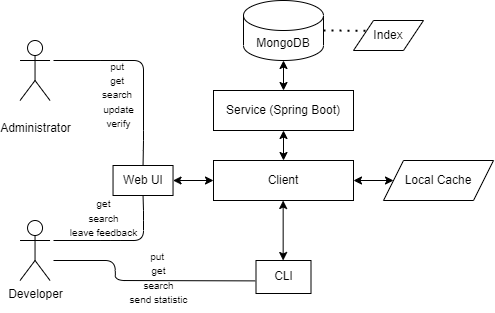
\includegraphics[width=0.52\textwidth]{arch}}
    \caption{Client-server application.}
    \label{fig:architecture}
\end{figure}

As for an administrator of the system, he can limit the number of
uploaded patterns, specify some restrictions for the maximum amount of
uploaded data or just prohibit the upload to a specific user. Another
available functionality for an administrator is an opportunity to
modify existing documents by merging some of them, updating and
deleting.

Asking for upload the same documents is quite common for the process
of applying patterns from them, therefore it was decided to develop a
local client cache. Further details of the operation of the cache will
be given here:
\begin{itemize}
    \item It would be great to get a document from the
local cache if there is no connection to the service and the necessary
item exists.
    \item If the service is available and the item exists in the
local memory, it is necessary to check that the data has not expired
(for example, the local timestamp of the document and the timestamp of
the deleted document match).
    \item If cached documents have been modified locally in some way
and these changes have been transferred to the service, it is
necessary to delete such documents from the local cache.
    \item There is no need to validate the local cache very often. A
document can be considered fresh (e.g. not expired) if it was
updated within the specified time interval (for example, 1 hour).
Immediate refreshing of documents is not critical. It is better to
avoid redundant requests to the server.
\end{itemize}

The most common way of using the service is to download existing
documents from the storage. A user has several filters to obtain only
necessary documents with patterns. For example, he can specify the
full description of the library to be replaced during migration, and
the same for the second one. Another available filter is to get all
the data for a specific programming language. After downloading
documents from a centralized repository, patterns are applied using
the Patternika tool \cite{c1}. 

\section{Expected results}

TODO: let's summarize the final expected result - the output will be a
program with the features listed above that meets the requirements

\section{Conclusion}

Automation of modifying source code is becoming more popular
in the world of software development as it allows to reduce the amount
of monotonous work. This helps to the improve the quality of the source
code and reduce the influence of the human factor on the occurrence of
errors. Following these trends, the number of patterns increases, covering
more and more cases. In this paper, it is proposed to develop a
centralized repository with patterns to distribute them among different
teams and developers. A client-server application with an opportunity of administering it is the target of this work.

\addtolength{\textheight}{-12cm}   % This command serves to balance the column lengths
                                  % on the last page of the document manually. It shortens
                                  % the textheight of the last page by a suitable amount.
                                  % This command does not take effect until the next page
                                  % so it should come on the page before the last. Make
                                  % sure that you do not shorten the textheight too much.

%%%%%%%%%%%%%%%%%%%%%%%%%%%%%%%%%%%%%%%%%%%%%%%%%%%%%%%%%%%%%%%%%%%%%%%%%%%%%%%%



%%%%%%%%%%%%%%%%%%%%%%%%%%%%%%%%%%%%%%%%%%%%%%%%%%%%%%%%%%%%%%%%%%%%%%%%%%%%%%%%



%%%%%%%%%%%%%%%%%%%%%%%%%%%%%%%%%%%%%%%%%%%%%%%%%%%%%%%%%%%%%%%%%%%%%%%%%%%%%%%%



\begin{thebibliography}{99}
\bibitem{c1} Andrei Tatarnikov et al., “Patternika: A
Pattern-Mining-Based Tool for Automatic Library Migration”,
Proceedings of the 32nd International Symposium on Software
Reliability Engineering (ISSRE 2021), Wuhan, China, 2021, p. 6.
\bibitem{c2} J. Bader, A. Scott, M. Pradel, and S. Chandra, “Getafix:
Learning to fix bugs automatically”, Proceedings of the ACM on Programming
Languages, p. 19, 2019.
\bibitem{c3} R. Rolim, G. Soares, R. Gheyi, and L. D’Antoni, “Learning
quick fixes from code repositories,” p. 12, 2018.
\end{thebibliography}

\end{document}
